\documentclass[8pt, t,
aspectratio=169,% for widescreen (16:9) presentations
%aspectratio=43,% for traditional (4:3) presentations
%handout%
]{beamer}


%%%%%%%%%%%%%%%%%%%%%%%%%%%%%%%%%% mode options %%%%%%%%%%%%%%%%%%%%%%%%%%%%%%%%

\mode<presentation>{\usetheme{uniS}}

% define a few pictures used throughout the slides
\pgfdeclareimage[height=1.1\paperheight]{background}{bg.jpg}  % background picture for title slide
\pgfdeclareimage[height=1cm]{unilogo}{unilogo.pdf} % UniS logo for title slide
\pgfdeclareimage[height=1cm]{unilogow}{unilogo_w.pdf} % (white) UniS logo for final slide
\pgfdeclareimage[width=2.5cm]{speaker}{speaker.jpg} % speaker photo for final slide


%%%%%%%%%%%%%%%%%%%%%%%%%%%%%%%%%% misc stuff %%%%%%%%%%%%%%%%%%%%%%%%%%%%%%%%%%

% automatically display \sectionpage at beginning of every \section{}
\AtBeginSection[]{%
\begin{frame}[plain]
  \sectionpage
\end{frame}
% uncomment block in order to display toc after every sectionpage
%\usepackage{multicol}
%\begin{frame}[c, plain]
%  \begin{footnotesize}
%    \begin{center}
%      \begin{minipage}{.75\textwidth}
%        \begin{multicols}{2}
%          \tableofcontents[currentsection]
%        \end{multicols}
%      \end{minipage}
%    \end{center}
%  \end{footnotesize}
%\end{frame}
}


%%%%%%%%%%%%%%%%%%%%%%%%%%%%%%%%%%%% setup %%%%%%%%%%%%%%%%%%%%%%%%%%%%%%%%%%%%%

\title[\LaTeX-Folien im CD der UniS]{\LaTeX-Vortragsfolien\\im Corporate Design der\\Universität Stuttgart}
\author[Dr.-Ing. Christian Senger]{Dr.-Ing.\\Christian Senger}
\institute{Institut für Nachrichtenübertragung (INÜ), Universität Stuttgart}

%%%%%%%%%%%%%%%%%%%%%%%%%%%%%%%%%%% slides %%%%%%%%%%%%%%%%%%%%%%%%%%%%%%%%%%%%%

\begin{document}

\begin{frame}[plain]
  \titlepage
\end{frame}

\section{Einführung}

\begin{frame}{Corporate Design-Folien}
  \begin{columns}[c]
    \begin{column}{.7\textwidth}
      \begin{itemize}
        \item Farben, Schriften und Formate gemäß Corporate Design vordefiniert
        \item Basiert auf der \LaTeX Beamer-Klasse
        \item Vorlage wird in den nächsten Monaten noch weiterentweickelt
        \item Bilder können bspw. über \texttt{\textbackslash includegraphics} eingebunden werden
        \item \glqq Einbauen\grqq{} von Formeln wie gewohnt: $e=mc^2$ oder bspw.
          \begin{equation*}
            \sum_{k=0}^{n-1} ar^k=a\frac{1-r^n}{1-r}
          \end{equation*}
        \item Beamer-Blöcke können verwendet werden, sind aber \emph{nicht} Corporate Design-konform
        \item Einige Hinweise auf weitere Funktionialität im Quelltext von \texttt{example.tex}, bspw.
          Umschaltung zwischen 4:3 und 16:9-Format
        \item Es müssen die Schriftarten \alert{UniversforUniS65Bd-Regular} und
          \alert{UniversforUniS45LtObl-Rg} installiert sein (erhältlich über ILIAS)
        \item Übersetzen mit \texttt{xelatex}, ggfs. zweimal
      \end{itemize}
    \end{column}
    \begin{column}{.3\textwidth}
      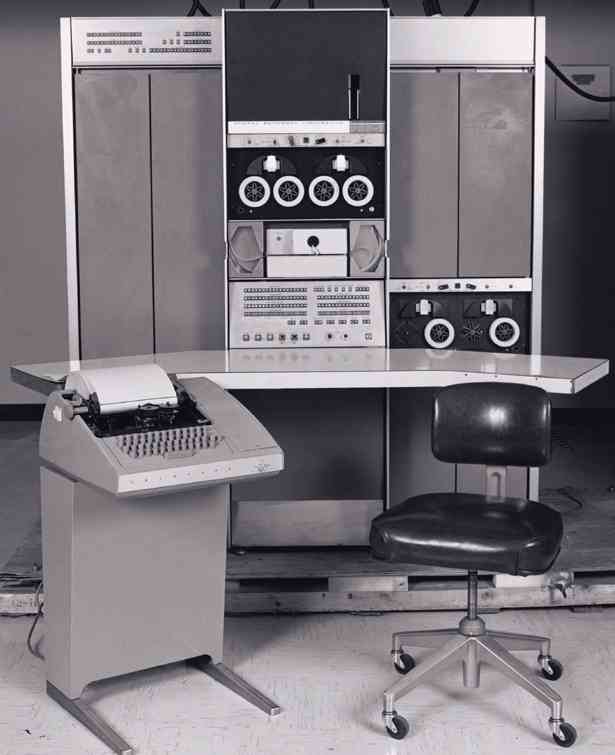
\includegraphics[width=\textwidth]{fig/pdp7.jpg}
    \end{column}
  \end{columns}

  \photocredit{DEC PDP-7 Promo-Material}

\end{frame}


%%%%%%%%%%%%%%%%%%%%%%%%%%%%%%%%% final slide %%%%%%%%%%%%%%%%%%%%%%%%%%%%%%%%%%
%\finalslide{<<email>>}{<<tel>>}{<<fax>>}
\finalslide{senger@inue.uni-stuttgart.de}{+49-711-685 679 42}{+49-711-685 579 42}

%%%%%%%%%%%%%%%%%%%%%%%%%%%%%%%%%%% appendix %%%%%%%%%%%%%%%%%%%%%%%%%%%%%%%%%%%

%\appendix
%
%\begin{frame}{References}
%   \renewcommand*{\bibfont}{\tiny}
%   \printbibliography
%\end{frame}

\end{document}
